\Class{Wilder}
{Power flows through my veins, beckoning to be released. But if I do, it burns!}{Garath, gith wilder}

For most wilders, psionic power is not a choice, but a discovery. Some wilders discovered their mental powers in childhood or puberty. While psions train in the academies to harness their abilities, wilders tend to discover their powers accidentally and without training. Most wilders never work to harness their powers, lacking the time, inclination or will to further their training. Low-level wilders often think of their power as a handy ``gift'' or ``knack'', rather than a trait that defines them. Generally, only the more focused and powerful will actually identify themselves as ``wilders''.

Wilders often first release their abilities while under great stress. Even as they progress, stress or excitement can flood through a wilder, allowing a display of power beyond his normal range of ability.

\PsychicTable{The Wilder}{
1  & +0         & +0 & +0 & +2  & Wild surge +1, psychic enervation & 2   & 1  & 1st \\
2  & +1         & +0 & +0 & +3  & Elude touch                       & 6   & 2  & 1st \\
3  & +2         & +1 & +1 & +3  & Wild surge +2                     & 11  & 2  & 1st \\
4  & +3         & +1 & +1 & +4  & Surging euphoria +1               & 19  & 3  & 2nd \\
5  & +3         & +1 & +1 & +4  & Volatile mind (1 power point)     & 27  & 3  & 2nd \\
6  & +4         & +2 & +2 & +5  &                                   & 36  & 4  & 3rd \\
7  & +5         & +2 & +2 & +5  & Wild surge +3                     & 47  & 4  & 3rd \\
8  & +6/+1      & +2 & +2 & +6  &                                   & 58  & 5  & 4th \\
9  & +6/+1      & +3 & +3 & +6  & Volatile mind (2 power points)    & 71  & 5  & 4th \\
10 & +7/+2      & +3 & +3 & +7  &                                   & 84  & 6  & 5th \\
11 & +8/+3      & +3 & +3 & +7  & Wild surge +4                     & 98  & 6  & 5th \\
12 & +9/+4      & +4 & +4 & +8  & Surging euphoria +2               & 113 & 7  & 6th \\
13 & +9/+4      & +4 & +4 & +8  & Volatile mind (3 power points)    & 129 & 7  & 6th \\
14 & +10/+5     & +4 & +4 & +9  &                                   & 145 & 8  & 7th \\
15 & +11/+6/+1  & +5 & +5 & +9  & Wild surge +5                     & 162 & 8  & 7th \\
16 & +12/+7/+2  & +5 & +5 & +10 &                                   & 181 & 9  & 8th \\
17 & +12/+7/+2  & +5 & +5 & +10 & Volatile mind (4 power points)    & 199 & 9  & 8th \\
18 & +13/+8/+3  & +6 & +6 & +11 &                                   & 219 & 10 & 9th \\
19 & +14/+9/+4  & +6 & +6 & +11 & Wild surge +6                     & 239 & 10 & 9th \\
20 & +15/+10/+5 & +6 & +6 & +12 & Surging euphoria +3               & 260 & 11 & 9th \\
}

\begin{figure}[t!]
\centering
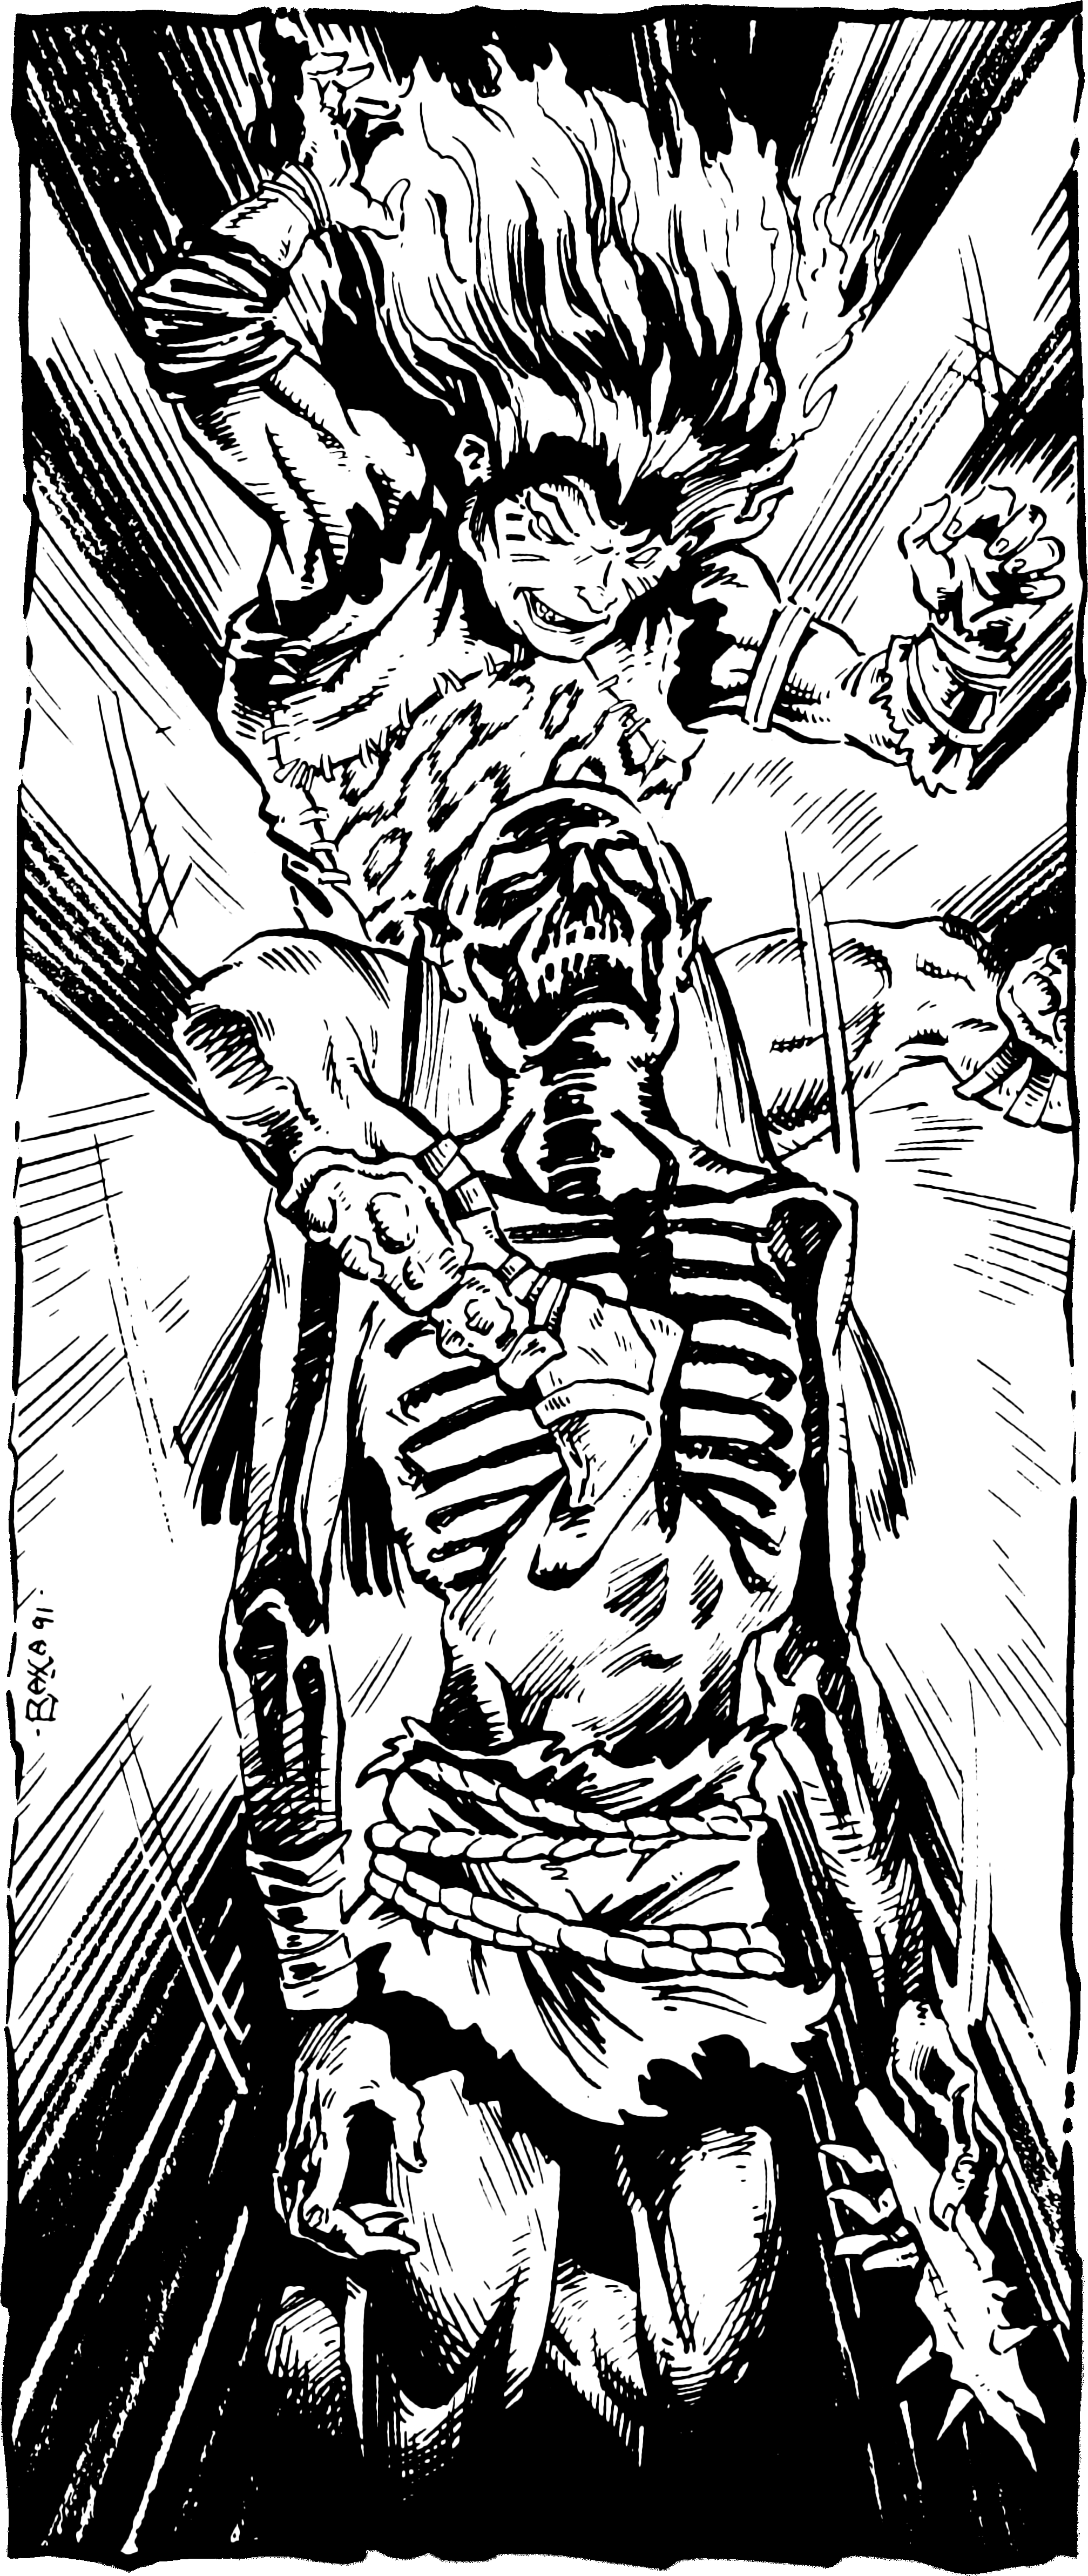
\includegraphics[width=\columnwidth]{images/psionic-1.png}
\WOTC
\end{figure}

\subsection{Making a Wilder}

Through experience, the wilder discovers supernatural powers that are an extension of his personality. Wilders know fewer powers than other manifesting classes, but their wild surge ability gives their powers greater flexibility. These surges are not without cost, however, and can have a great toll on the careless wilder.

\textbf{Races:} Psionic talent is common in the tablelands. Because of the limited access to psionic instruction, humans elves, halflings, and to a lesser extent, muls, are much more likely to be wilders than psions. Races that are less charismatic, less individualistic, and less prone to emotion, such as thri-kreen and dwarves rarely become wilders; more of them become psions or psychic warriors. The pterran culture glorifies the path of the psion, so wilders are rare. Half-giants tend to become wilders rather than psions, because even with psionic training, many half-giants lack the wit, Will, or focus to excel as psions.

\textbf{Alignment:} Though wilders have no inclinations towards good or evil, as a whole they tend to be chaotic.

\subsection{Game Rule Information}

\textbf{Hit Die:} d6.

\subsubsection{Class Skills}
\skill{Autohypnosis} (Wis), \skill{Balance} (Dex), \skill{Bluff} (Cha), \skill{Climb} (Str), \skill{Concentration} (Con), \skill{Craft} (Int), \skill{Escape Artist} (Dex), \skill{Intimidate} (Cha), \skill{Jump} (Str), \skill{Knowledge} (psionics) (Int), \skill{Listen} (Wis), \skill{Profession} (Wis), \skill{Psicraft} (Int), \skill{Sense Motive} (Wis), \skill{Spot} (Wis), \skill{Survival} (Wis), and \skill{Tumble} (Dex).

\textbf{Skill Points per Level:} 4 + Int modifier ($\times 4$ at 1st level).

\subsubsection{Class Features}

\textbf{Weapon and Armor Proficiency:} Wilders are proficient with all simple weapons, with light armor, and with shields (except tower shields).

\textbf{Power Points/Day:} A wilder's ability to manifest powers is limited by the power points she has available. Her base daily allotment of power points is given on \tabref{The Wilder}. In addition, she receives bonus power points per day if she has a high Charisma score (see \tabref{Ability Scores and Bonus Power Points}). Her race may also provide bonus power points per day, as may certain feats and items.

\textbf{Powers Known:} A wilder begins play knowing one wilder power of your choice. At every even-numbered class level after 1st, she unlocks the knowledge of new powers.

Choose the powers known from the wilder power list. (Exception: The feat \feat{Expanded Knowledge} do allow a wilder to learn powers from the lists of other classes.) A wilder can manifest any power that has a power point cost equal to or lower than her manifester level.

The total number of powers a wilder can manifest in a day is limited only by her daily power points.

A wilder simply knows her powers; they are ingrained in her mind. She does not need to prepare them (in the way that some spellcasters prepare their spells), though she must get a good night's sleep each day to regain all her spent power points.

The Difficulty Class for saving throws against wilder powers is 10 + the power's level + the wilder's Charisma modifier.

\textbf{Maximum Power Level Known:} A wilder begins play with the ability to learn 1st-level powers. As she attains higher levels, she may gain the ability to master more complex powers.

To learn or manifest a power, a wilder must have a Charisma score of at least 10 + the power's level.

\textbf{Wild Surge (Su):} A wilder can let her passion and emotion rise to the surface in a wild surge when she manifests a power. During a wild surge, a wilder gains phenomenal psionic strength, but may harm herself by the reckless use of her power (see Psychic Enervation, below).

A wilder can choose to invoke a wild surge whenever she manifests a power. When she does so, she gains +1 to her manifester level with that manifestation of the power. The manifester level boost gives her the ability to augment her powers to a higher degree than she otherwise could; however, she pays no extra power point for this wild surge. Instead, the additional 1 power point that would normally be required to augment the power is effectively supplied by the wild surge.

Level-dependent power effects are also improved, depending on the power a wilder manifests with her wild surge.

This improvement in manifester level does not grant her any other benefits (psicrystal abilities do not advance, she does not gain higher-level class abilities, and so on).

She cannot use the \feat{Overchannel} psionic feat and invoke her wild surge at the same time.

At 3rd level, a wilder can choose to boost her manifester level by two instead of one. At 7th level, she can boost her manifester level by up to three; at 11th level, by up to four; at 15th level, by up to five; and at 19th level, by up to six.

In all cases, the wild surge effectively pays the extra power point cost that is normally required to augment the power; only the unaugmented power point cost is subtracted from the wilder's power point reserve.

\textbf{Psychic Enervation (Ex):} Pushing oneself by invoking a wild surge is dangerous. Immediately following each wild surge, a wilder may be overcome by the strain of her effort. The chance of suffering psychic enervation is equal to 5\% per manifester level added with the wild surge.

A wilder who is overcome by psychic enervation is dazed until the end of her next turn and loses a number of power points equal to her wilder level.

\textbf{Elude Touch (Ex):} Starting at 2nd level, a wilder's intuition supersedes her intellect, alerting her to danger from touch attacks (including rays). She gains a bonus to Armor Class against all touch attacks equal to her Charisma bonus; however, her touch AC can never exceed her Armor Class against normal attacks.

\textbf{Surging Euphoria (Ex):} Starting at 4th level, when a wilder uses her wild surge ability, she gains a +1 morale bonus on attack rolls, damage rolls, and saving throws for a number of rounds equal to the intensity of her wild surge.

If a wilder is overcome by psychic enervation following her wild surge, she does not gain the morale bonus for this use of her wild surge ability.

At 12th level, the morale bonus on a wilder's attack rolls, damage rolls, and saving throws increases to +2. At 20th level, the bonus increases to +3.

\textbf{Volatile Mind (Ex):} A wilder's temperamental mind is hard to encompass with the discipline of telepathy. When any telepathy power is manifested on a wilder of 5th level or higher, the manifester of the power must pay 1 power point more than he otherwise would have spent.

The extra cost is not a natural part of that power's cost. It does not augment the power; it is simply a wasted power point. The wilder's volatile mind can force the manifester of the telepathy power to exceed the normal power point limit of 1 point per manifester level. If the extra cost raises the telepathy power's cost to more points than the manifester has remaining in his reserve, the power simply fails, and the manifester exhausts the rest of his power points.

At 9th level, the penalty assessed against telepathy powers manifested on a wilder is increased to 2 power points. At 13th level, the penalty increases to 3 power points, and at 17th level it increases to 4 power points.

As a standard action, a wilder can choose to lower this effect for 1 round.

\subsection{Playing a Wilder}
As a wilder, you adventure to practice your abilities and gain further understanding and mastery about the Will. You are very passionate about your powers, and you often push yourself to your limits with your wild surges, but you are not blind to its dangers.

\subsubsection{Religion}
Although wilders, like psions, draw their energies from within, wilder powers require less focus and discipline, so wilders are as likely as any other Athasian to be religious. A wilders religion can have a great impact on his power selection. A wilder who worships fire, for example, often discovers powers that involve light, heat or flame.

\subsubsection{Other Classes}
Wilder's opinions vary wildly. Some wilders view psions with awe, respecting the psion's greater knowledge and control; others chafe under the psion's perceived superiority complex.

\subsubsection{Combat}
In combat, you use your impressive array of psionic powers for both attack and defense against your enemies and opponents, just as any other psionicist would. Of course, as a wilder, you can call upon swells of psionic potential that other psionicists cannot access in the form of wild surges.

\subsubsection{Advancement}
Your interest on psionics is more than academic---it has been your motivating force for years. Perhaps you became a wilder after witnessing one destroying an entire village during one of his surges, or you vowed to gain control of the power you first displayed in your puberty every time you got were angered. Whatever the case, since the day you first became a wilder, you've worked to master a power more primal than spells and stronger than steel.

The powers you choose strongly shape your abilities. You are heavily invested in combat prowess as a result of the erratic and emotional nature of your power, but you have some flexibility in how you learn your powers. If you choose only offensive powers, you will have few defenses and limited versatility beyond combat, but you'll be devastating even in dire situations. If you focus on other powers, you will have more options outside a fight, but you might have only area attacks that could accidentally hurt a friend.

\subsection{Starting Packages}
\subsubsection{The Battle Wilder}
Mul Wilder

\textbf{Ability Scores:} Str 17, Dex 8, Con 16, Int 10, Wis 12, Cha 13.

\textbf{Skills:} \skill{Concentration}, \skill{Intimidate}, \skill{Psicraft}.

\textbf{Languages:} Common.

\textbf{Feat:} \feat{Combat Manifestation}.

\textbf{Weapons:} Longspear (1d8/$\times$3).

\textbf{Armor:} Scale mail (+4 AC).

\textbf{Other Gear:} Standard adventurer's kit, 20 cp.

\subsubsection{The Blaster}
Human Wilder

\textbf{Ability Scores:} Str 8, Dex 14, Con 13, Int 12, Wis 10, Cha 15.

\textbf{Skills:} \skill{Concentration}, \skill{Intimidate}, \skill{Knowledge} (psionics), \skill{Psicraft}.

\textbf{Languages:} Common.

\textbf{Feat:} \feat{Lightning Reflexes}, \feat{Psionic Endowment}.

\textbf{Weapons:} Spear (1d8/$\times$3, 6 m)

Light crossbow with 20 bolts (1d8/19--20, 24 m).

\textbf{Armor:} Leather (+2 AC).

\textbf{Other Gear:} Standard adventurer's kit, 26 cp.

\subsubsection{The Sharpshooter}
Halfling Wilder

\textbf{Ability Scores:} Str 6, Dex 16, Con 13, Int 12, Wis 10, Cha 15.

\textbf{Skills:} \skill{Concentration}, \skill{Intimidate}, \skill{Spot} (cc).

\textbf{Languages:} Halfling.

\textbf{Feat:} \feat{Point Blank Shot}.

\textbf{Weapons:} Spear (1d8/$\times$3, 6 m)

Light crossbow with 20 bolts (1d8/19--20, 24 m).

\textbf{Armor:} Leather (+2 AC).

\textbf{Other Gear:} Standard adventurer's kit, 26 cp.

\subsection{Wilders on Athas}
\Quote{Something seemed strange the second I saw Nakua's face. It's odd. He acted like a different person. My friend Kuko asked him if he was really Nakua or if he was someone else. And those were his last words}{Ekee, elven dancer}

Psionic is very common on Athas, and wilders can be widely found in the Tablelands, representing psionic energy in its most raw state, and change for change's sake. Neutral wilders are rare, but such characters become famous within the ranks of their comrades, since their vision is unclouded by moral concerns.

Wilders know that using psionic powers can be strenuous, and the limit of a character's endurance is his Will. Eventually, even the most powerful of masters becomes exhausted and must rest to replenish his strength. When wounds and exhaustion cloud the vision and the mind swims in delirium, only the greatest wilders possess the Will to continue using their powers.

\subsubsection{Daily Life}

Wilders spend their days in travel and contemplation, with an occasional rant and wild outburst (usually against the foes an adventurer comes across). They enjoy talking about their psionic abilities and about their life philosophies.

\subsubsection{Notables}

The xenophobic Kenkus (FFN 126) are the race to most commonly sport wilders, although no one knows for sure why. Elves, due to their chaotic nature, also seem to have a higher rate of wilders in their milieu.

\subsubsection{Organizations}

A wilder's path is his own to thread, since no overarching organization exists to recruit you into its ranks. Most wilders are just too erratic and freedom-loving to join one, anyway.

\subsubsection{NPC Reactions}

Most people do not understand the difference between a psion and a wilder, so their attitudes span the spectrum. Psions NPC attitudes range from indifferent to unfriendly, although most \class{Psiologists} tend to have their attitude bent towards hostile.

\subsubsection{Wilder Lore}

Characters with ranks in \skill{Knowledge} (psionics) can research wilders to learn more about them. When a character makes a skill check, read or paraphrase the following, including the information from lower DCs.

\textbf{DC 10:} A wilder is a kind of psionicist that can trigger a surge of psionic power beyond control.

\textbf{DC 15:} Wilders usually become very weak, both physically and mentally, after unleashing their psionic surges.

\textbf{DC 20:} Experienced wilders learn how to further tap into their Will and manage to also strengthen their bodies while surging.